
\section{Transformace souřadníc a jejích kovariančních matíc medzi vybranými souřadnicovými soustavami}

\subsection{ECEF $\rightarrow$ ENU}
Předpokládejme, že v tomto příkladu je uvažovaný rotační elipsoid (například WGS-84 nebo GRS-80) geocentrický, to znamená, že střed elipsoidu se nachází ve středu zemského tělesa. Transformace souřadnic pak mezi zemským geocentrickým systémem souřadnic (xyz) a lokálním topocentrickým (nebo také lokálním geodetickým - enu) systémem může být vyjádřený předpisem \cite{Soler1998}

\begin{equation}
\begin{bmatrix}
e \\
n \\
u
\end{bmatrix} = 
\mathbf{C}_{enu}^{xyz}
\begin{bmatrix}
x \\
y \\
z
\end{bmatrix}.
\label{rov:ecef2enu1}
\end{equation}

Pro popis transformace mezi uvedenými systémy si potřebujeme odvodit transformační matici, v tomto případě takzvanou rotační matici. Vycházejme z rovnice \ref{rov:generRotMat}. Rotační matici pak zostavíme pro rotaci v prostoru a to pomocí jednoduchých rotací v každé ose samostatně.

Rotační matice kolem osy \textit{z} ve směru hodinových ručiček nabude tvar
\begin{equation}
\mathbf{R_{3}}\left(\theta\right) = 
\begin{bmatrix}
\cos{\left(\theta\right)} & \sin{\left(\theta\right)} & 0 \\
-\sin{\left(\theta\right)} & \cos{\left(\theta\right)} & 0 \\
0 & 0 & 1
\end{bmatrix},
\end{equation}
přičemž rotace kolem osy \textit{z} je $\cos{\left(\theta_{z, w} \right)} = \cos{\left(0\right)} = 1$, protože úhel mezi osama \textit{z} a \textit{w}, které jsou v tomto přikladě totožné, je roven nule. Dále platí, že kosinus úhlu $ \cos{\left(\theta_{z, u} \right)}= \cos{\left(90\right)} = 0 $, protože \textit {z} a \textit {u} jsou na sebe kolmé. Stejně tento předpoklad platí i pro $\cos{\left(\theta_{z,v}\right)}$, $\cos{\left(\theta_{x,w}\right)}$ a $\cos{\left(\theta_{y,w}\right)}$.

Analogicky postup bude platit i pro ostatní dvě rotace a tedy rotace kolem osy \textit{x} je
\begin{equation}
\mathbf{R_{1}}\left(\theta\right) = 
\begin{bmatrix}
1 & 0 & 0 \\
0 &  \cos{\left(\theta\right)} & \sin{\left(\theta\right)} \\
0 & -\sin{\left(\theta\right)} & \cos{\left(\theta\right)} \\
\end{bmatrix},
\end{equation}
a kolem osy \textit{y}
\begin{equation}
\mathbf{R_{2}}\left(\theta\right) = 
\begin{bmatrix}
\cos{\left(\theta\right)} & 0 & -\sin{\left(\theta\right)} \\
0 & 1 & 0 \\
\sin{\left(\theta\right)} & 0 & \cos{\left(\theta\right)} \\
\end{bmatrix},
\end{equation}

Vyjádření transformační matice $\mathbf {C}_{enu}^{xyz} $ mezi dvěma pravoúhlými kartézskymi souřadnicovými systémy ECEF a ENU je založen na součinu dvou rotací, konkrétně:
\begin{enumerate}
\item rotaci kolem osy \textit{z} o úhel $\pi/2 + \lambda $ a
\item rotaci kolem osy \textit{y} o úhel $\pi/2 - \varphi $,
\end{enumerate}
kde úhlové stupně $\lambda$, respektíve $\varphi$ geograficky představují stupeň otočení jedné soustavy od druhé ve směru zeměpisné délky ($\lambda$) a ve směru zeměpisné šířky ($\varphi$).

Potom transformace mezi systémy se dá vyjádřit ve tvaru

\begin{equation}
\begin{bmatrix}
e \\
n \\
u
\end{bmatrix} =
\mathbf{R_{1}}\left(\pi/2-\varphi\right)\mathbf{R_{3}}\left(\pi/2+\lambda\right)
\begin{bmatrix}
x \\
y \\
z
\end{bmatrix} =
\begin{bmatrix}
-\sin{\left(\lambda\right)} & \cos{\left(\lambda\right)} & 0 \\
-\cos{\left(\lambda\right)}\sin{\left(\varphi\right)} & -\sin{\left(\lambda\right)}\sin{\left(\varphi\right)} & \cos{\left(\varphi\right)} \\
\cos{\left(\lambda\right)}\cos{\left(\varphi\right)} & \sin{\left(\lambda\right)}\cos{\left(\varphi\right)} & \sin{\left(\varphi\right)}
\end{bmatrix}
\begin{bmatrix}
x \\
y \\
z
\end{bmatrix}.
\label{rov:ecef2enu2}
\end{equation}

Z předchozího zápisu plyne, že během rotace pravoúhlých souřadnicových soustav předpokládáme, že počátky souřadnic jsou shodné. V případě, že počátek, například soustavy ENU umístíme na povrch referenčního tělesa (elipsoid případně sféry), je zapotřebí doplnit posun mezi soustavami. Potom rovnice \ref{rov:ecef2enu2} nabude tvar

\begin{equation}
\begin{bmatrix}
e \\
n \\
u
\end{bmatrix} =
\mathbf{R}
\begin{bmatrix}
x - x_{0} \\
y - y_{0} \\
z - z_{0}
\end{bmatrix},
\label{rov:ecef2enu22}
\end{equation}

Při transformaci kovariančných matic vycházejme z předpokladu a definice Zákona hromadění středních chyb. Budeme vycházet z článku Transformace kovariančních matic. Předpokládejme, že kovariančná matice souřadnic soustavy ze které chceme transformovat $\Sigma_{xyz}$, je známá a to například jako důsledek numerického výpočtu (regrese, vyrovníní, estimace souřadnice a jejich přesností atp.). Hlavní úlohou je v tomto kroku vyčíslit Jakobiho matici. Rozepsáním matic pro jednotlivé veličiny \textit{e,n,u} z předchozích rovnic a následným parciálním derivovaním podle veličin \textit{x,y,z} snadno zjistíme, že Jakob matice $\mathbf{J}$ je totožná s rotační matici $\mathbf{R}$ a tedy
\begin{equation}
\mathbf{J} = \mathbf{R}.
\end{equation}
Kovarianční matice souřadníc systému ENU pak nadobude tvaru
\begin{equation}
\mathbf{\Sigma}_{enu} = \mathbf{J}\mathbf{\Sigma}_{xyz}\mathbf{J}^{T} = \mathbf{R}\mathbf{\Sigma}_{xyz}\mathbf{R}^{T}.
\end{equation}

\subsubsection{Příklad transformace z ECEF $\rightarrow$ ENU}

Nechť bod A je vyjádřen v souřadnicích souřadného systému ECEF a hodnoty souřadnic jsou:
\begin{itemize}
\item $x = 4198944.6161$ m
\item $y = 174747.2383$ m
\item $z = 4781886.8769$ m
\end{itemize}

Mějme bod B, jehož geodetické souřadnice jsou $ \varphi = 48.8862 deg$, $\lambda = 2.3343 deg$ a geodetická výška je $ h = 174.5217 m $. Úhlové souřadnice použijeme jednak k natočení souřadných soustav (viz rotační matice v rovnici \ref{rov:ecef2enu2}) a společně se zadanou elipsoidickou výškou, k umístění počátku ENU soustavy, který umístíme nad povrch rotačního elipsoidu. Úkolem je vyjádřit souřadnice bodu \textit{A} v soustavě ENU a s přihlédnutím definovaného počátku ENU soustavy v bodě B.

Vektor pravoúhlých souřadnic bodu B, tj $ \left(x_{0}, y_{0}, z_{0} \right)$ získáme transformací GEOD2ECEF(). ENU souřadnice bodu A s přihlédnutím k umístění počátku ENU soustavy v bodě B a vypočítané podle \ref{rov:ecef2enu22}, jsou:
\begin{itemize}
\item $e = 3579.4232 $ m
\item $n = -688.3514 $ m
\item $u = -51.0524 $ m.
\end{itemize}

Pseudokód Matlab funkce ecef2enu(), která je implementováná v package +Geo je stručně popsaná v příloze \ref{appEcef2Enu}.


\subsection{ENU $\rightarrow$ ECEF}


Jednou z vlastností rotačných matíc je tá, podle které $\mathbf{R}\left(\theta\right)^{-1} = \mathbf{R}\left(-\theta\right) = \mathbf{R}\left(\theta\right)^{T}$. Z toho plyne, že zápis pro inversnou tranformaci je

\begin{equation}
\begin{bmatrix}
x \\
y \\
z
\end{bmatrix} =
\mathbf{R_{3}}\left(-\left(\pi/2+\lambda\right)\right)\mathbf{R_{1}}\left(-\left(\pi/2-\varphi\right)\right)
\begin{bmatrix}
e \\
n \\
u
\end{bmatrix} = 
\begin{bmatrix}
-\sin{\left(\lambda\right)} & -\cos{\left(\lambda\right)}\sin{\left(\varphi\right)} & \cos{\left(\lambda\right)}\cos{\left(\varphi\right)} \\
 \cos{\left(\lambda\right)} & -\sin{\left(\lambda\right)}\sin{\left(\varphi\right)} & \sin{\left(\lambda\right)}\cos{\left(\varphi\right)} \\
 0  &  \cos{\left(\varphi\right)} & \sin{\left(\varphi\right)} 
\end{bmatrix}
\begin{bmatrix}
e \\
n \\
u
\end{bmatrix}.
\label{rov:ecef2enu3}
\end{equation}
a po doplnění předpokaldu translace počátku souřadné soustavy, rovnici \ref{rov:ecef2enu3} doplníme do tvaru

\begin{equation}
\begin{bmatrix}
x \\
y \\
z
\end{bmatrix} =
\begin{bmatrix}
x_{0} \\
y_{0} \\
z_{0}
\end{bmatrix} + 
\mathbf{R}^{T}
\begin{bmatrix}
e \\
n \\
u
\end{bmatrix},
\label{rov:ecef2enu33}
\end{equation}
kde pravoúhlé souřadnice vektoru $\mathbf{r}_{0}=\left[x_{0}, y_{0}, z_{0} \right]$ získáme transformací zeměpisných souřadnic posunutého počátku například ENU soustavy ($\varphi$, $\lambda$, $hel$) do systému geocentrických kartézskych souřadnic (například systému ECEF).

Odhad kovarianční matice $\Sigma_{xyz}$ geocentrických pravoyhlých souřadníc kopíruje postup jako v případe odhadu matice $\Sigma_{enu}$, no s tým rozdílem, že zde je 
\begin{equation}
\mathbf{J} = \mathbf{R}^{-1},
\end{equation}
respektíve vzhledem k vlastnostem matice rotace \textbf{R}
\begin{equation}
\mathbf{J} = \mathbf{R}^{T}.
\end{equation}
Pro $\Sigma_{xyz}$ pak dostaneme
\begin{equation}
\mathbf{\Sigma}_{xyz} = \mathbf{J}\mathbf{\Sigma}_{enu}\mathbf{J}^{T}..
\end{equation}

\subsubsection{Příklad transformace z ENU $\rightarrow$ ECEF}

V tomto příkladě bude naší úlohou přezentovat inverzní transformaci, no vycházejme z výsledků výpočtu polohy bodu v ENU soustavě souřadnic, t.j. souřadníc pro bod B v předcházejícim příkladě. Jeho souřadnice jsou:

\begin{itemize}
\item $e = 3579.4232$ m
\item $n = -688.3514$ m
\item $u = -51.0524$ m.
\end{itemize}


Dle rovnice \ref{rov:ecef2enu33}, ECEF XYZ souřadnice bodu A jsou:
\begin{itemize}
\item $x = 4198944.6161$ m
\item $y = 174747.2383$ m
\item $z = 4781886.8769$ m.
\end{itemize}

Pseudokód Matlab funkce enu2ecef(), která je implmentováná v package +Geo Package je obsahem přílohy \ref{appEnu2Ecef}

\subsection{GEOD $\rightarrow$ ECEF}

Aby sme odvodili základní vzorce pro trnasformaci geodetických souřadníc na geocentrické pravouhlé kartézské souřadnice, je potřeba si vysvětlit základní geometrii mezi těmito souřadnicovými soustavami. V textu se budeme držet kompletního odvození a prepisu tak, jak je prezentován v kapitole 1.2 skriptu \cite{Cimbalnik1997}.

%\subsubsection{Vztah mezi geodetickou šířkou $\varphi$ bodu \textit{P} a jeho souřadnicemi \textit{x, y} v rovině meridiánové elipsy}

\begin{figure}[ht!]
\begin{center}

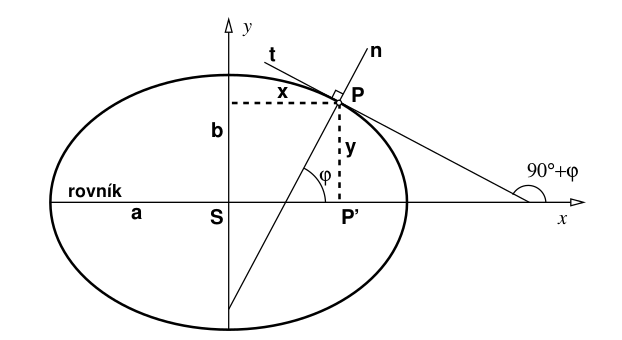
\includegraphics[width=0.60\textwidth]{FIG/CimbalnikObr1-14}
\caption{$\varphi$ $\rightarrow$ $\left(x, y\right)$. Obrázek je převzat z \cite{Cimbalnik1997}.}
\label{fig:cim114}
\end{center}
\end{figure}

Na obr. \ref{fig:cim114} svírá normála \textit{n} v bode \textbf{P} k elipse s 
velkou poloosou \textit{a} (s osou \textit{x} ) úhel $\varphi$ (geodetická šířka 
bodu \textbf{P} ). Odpovdidající tečna \textit{t} svíra s kladným směrem osy 
\textit{x} úhel $90^{\circ} + \varphi$ a její směrnice \textit{k} je dána vzorcem

\begin{equation}
k = \dfrac{dy}{dx} = \tan{\left(90^{\circ} + \varphi\right)} = -\cot{\left(\varphi\right)}.
\end{equation}
Diferencovaním rovnice meridiánové elipsy

\begin{equation}
\dfrac{x^{2}}{a^{2}} + \dfrac{y^{2}}{b^{2}} -1 = 0
\end{equation}
dostaneme

\begin{equation}
\dfrac{2xdx}{a^{2}} + \dfrac{2ydy}{b^{2}} = 0
\end{equation}
a odtud

\begin{equation}
\dfrac{dy}{dx} = - \dfrac{b^{2}x}{a^{2}y}.
\end{equation}
Z předchádzejícich rovníc vyplývá

\begin{equation}
\cot{\left(\varphi\right)} = \dfrac{b^{2}x}{a^{2}y} = \dfrac{\cos{\left(\varphi\right)}}{\sin{\left(\varphi\right)}}.
\end{equation}
Po umocnění a úpravě

\begin{equation}
b^{4}x^{2}\sin^{2}{\left(\varphi\right)} - a^{4}y^{2}\cos^{2}{\left(\varphi\right)} = 0
\end{equation}
a dále víme, že

\begin{equation}
b^{2}x^{2} + a^{2}y^{2} - a^{2}b^{2} = 0.
\end{equation}
Řešením těchto dvou (pro $x^{2}, y^{2}$ lineárních) rovníc dostaneme

\begin{equation}
x =\dfrac{a^{2}\cos{\left(\varphi\right)}}{\sqrt{a^{2}\cos^{2}{\left(\varphi\right)} + b^{2}\sin^{2}{\left(\varphi\right)}}}
\end{equation}
a
\begin{equation}
y =\dfrac{b^{2}\sin{\left(\varphi\right)}}{\sqrt{a^{2}\cos^{2}{\left(\varphi\right)} + b^{2}\sin^{2}{\left(\varphi\right)}}}.
\end{equation}
Do jmenovatelu dosaďme $b^{2} = a^{2}\left(1-e^{2}\right)$, potom po úpravě dostaneme

\begin{equation}
x =\dfrac{a\cos{\left(\varphi\right)}}{\sqrt{1-e^{2}\sin^{2}{\left(\varphi\right)}}} = \dfrac{a\cos{\left(\varphi\right)}}{W}
\label{rov:cimbX}
\end{equation}
a
\begin{equation}
y =\dfrac{a\left(1-e^{2}\right)\sin{\left(\varphi\right)}}{\sqrt{1-e^{2}\sin^{2}{\left(\varphi\right)}}} = \dfrac{a\left(1-e^{2}\right)\sin{\left(\varphi\right)}}{W},
\label{rov:cimbY}
\end{equation}
kde 
$W = \sqrt{1-e^{2}\sin^{2}{\left(\varphi\right)}}$ je první geodetická funkce.

Polohu bodu \textit{P} na rotačním elipsoidu vyjadříme v pravouhlé soustavě souřadnic. Její počátek je v středu elipsoidu \textit{S}, osa \textit{Z} v ose rotace, osa \textit{X} v průsečníku roviny rovníku s rovinou nultého poledníku, osa \textit{Y} v rovnině rovníku kolmá na osu \textit{X} - tak jak je to znázorneno na obrázku \ref{fig:cim116}.

\begin{figure}[ht!]
\begin{center}

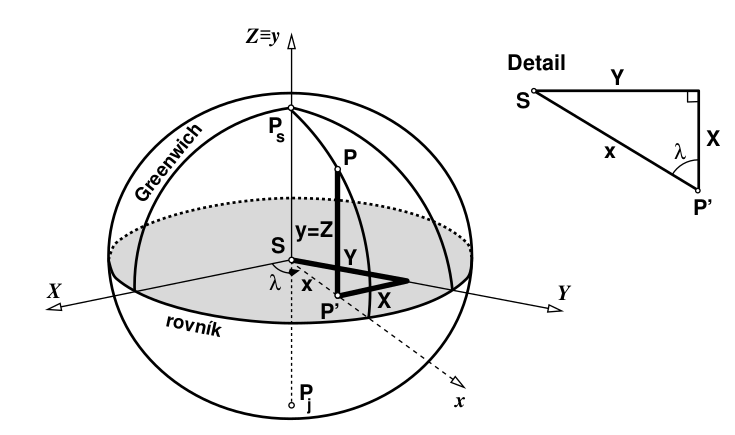
\includegraphics[width=0.60\textwidth]{FIG/CimbalnikObr1-16}
\caption{Prostorové pravouhlé souřadnice. Obrázek je převzat z \cite{Cimbalnik1997}.}
\label{fig:cim116}
\end{center}
\end{figure}

Bodem $P\left(\varphi, \lambda\right)$ prochází poledník $P_{s}-P-P_{j}-P_{s}$ o geodetické délke $\varphi$. V rovině tohto poledníku má bod \textit{P} pravouhlé souřadnice \textit{x, y}, odvozené vzorci \ref{rov:cimbX}, \ref{rov:cimbY}.

Podle obrázka \ref{fig:cim116} napíšeme pro souřadnice \textit{X, Y, Z} bodu \textit{P} vzorce

\begin{eqnarray}
X &=& x\cos{\left(\lambda\right)} \\
Y &=& x\sin{\left(\lambda\right)} \\
Z &=& y. 
\end{eqnarray}
Dosadíme-li do předchozích vzorců za x a y rovnice \ref{rov:cimbX} a \ref{rov:cimbY}, dostaneme

\begin{eqnarray}
X &=& \dfrac{a}{W}\cos{\left(\varphi\right)}\cos{\left(\lambda\right)} \\
Y &=& \dfrac{a}{W}\cos{\left(\varphi\right)}\sin{\left(\lambda\right)} \\
Z &=& \dfrac{a}{W}\left(1-e^{2}\right)\sin{\left(\varphi\right)}.
\end{eqnarray}
Uvážime-li vzorec pro příčný poloměr křivosti 
\begin{equation}
N = \dfrac{a}{W},
\end{equation}
potom geocentrické pravouhlé souřadnice bodu \textit{P} budou mít vzorce

\begin{equation}
\begin{bmatrix}
X\\
Y\\
Z
\end{bmatrix} = 
\begin{bmatrix}
N\cos{\left(\varphi\right)}\cos{\left(\lambda\right)}\\
N\cos{\left(\varphi\right)}\sin{\left(\lambda\right)}\\
N\left(1-e^{2}\right)\sin{\left(\varphi\right)}
\end{bmatrix}.
\end{equation}

V případe, že bod \textit{P} leží ve směru normály k elipsoidu ve výšce \textit{H} nad elipsoidem, pak předchozí rovnice budou
\begin{equation}
\begin{bmatrix}
X\\
Y\\
Z
\end{bmatrix} = 
\begin{bmatrix}
\left(N+H\right)\cos{\left(\varphi\right)}\cos{\left(\lambda\right)}\\
\left(N+H\right)\cos{\left(\varphi\right)}\sin{\left(\lambda\right)}\\
\left(N\left[1-e^{2}\right]+H\right)\sin{\left(\varphi\right)}
\end{bmatrix}.
\label{rov:geodEcef}
\end{equation}

Předpokládejme, že kovarianční matice souřadníc $\varphi, \lambda\ \text{a}\ H$, $\Sigma_{GEOD}$ je známá. Pro odhad kovarianční matice prostorových pravouhlých souřadníc \textit{X, Y, Z}, $\Sigma_{ECEF}$ budeme postupovať podle článku Transformace kovariančních matíc. Z článku víme, že úlohou je vyjádřít Jakobiho matici $\textbf{J}$. Derivovaním modelu rovníc \textit{X, Y, Z} z poslední rovníce podle veličín $\varphi, \lambda\ \text{a}\ H$, postupně dostaneme:

\begin{equation}
\mathbf{J} = 
\begin{bmatrix}
\dfrac{\partial X}{\partial \varphi} & \dfrac{\partial X}{\partial \lambda} & \dfrac{\partial X}{\partial H} \\
\dfrac{\partial Y}{\partial \varphi} & \dfrac{\partial Y}{\partial \lambda} & \dfrac{\partial Y}{\partial H} \\
\dfrac{\partial Z}{\partial \varphi} & \dfrac{\partial Z}{\partial \lambda} & \dfrac{\partial Z}{\partial H}.
\end{bmatrix}
\end{equation}
Pro jednotlivé zložky platí:

\begin{equation}
\dfrac{\partial X}{\partial \varphi} = \cos{\left(\lambda\right)}\left(\dfrac{\partial N}{\partial \varphi}\cos{\left(\varphi\right)}-\sin{\left(\varphi\right)}\left(N + H\right)\right),
\end{equation}

\begin{equation}
\dfrac{\partial X}{\partial \lambda} = -\left(N+H\right)\cos{\left(\varphi\right)}\sin{\left(\lambda\right)},
\end{equation}

\begin{equation}
\dfrac{\partial X}{\partial H} = \cos{\left(\varphi\right)}\cos{\left(\lambda\right)},
\end{equation}

%sin(lon) * (dNdLat * cos(lat) - vertRad * sin(lat) - hgt * sin(lat));
\begin{equation}
\dfrac{\partial Y}{\partial \varphi} = \sin{\left(\lambda\right)}\left(\dfrac{\partial N}{\partial \varphi} \cos{\left(\varphi\right)} - \sin{\left(\varphi\right)}\left(N + H\right)\right),
\end{equation}

\begin{equation}
\dfrac{\partial Y}{\partial \lambda} = \left(N+H\right)\cos{\left(\varphi \right)}\cos{\left(\lambda \right)},
\end{equation}

\begin{equation}
\dfrac{\partial Y}{\partial H} = \cos{\left(\varphi \right)}\sin{\left(\lambda \right)},
\end{equation}

\begin{equation}
\dfrac{\partial Z}{\partial \varphi} = \dfrac{b^{2}}{a^{2}}\left(\sin{\left( \varphi\right)} \dfrac{\partial N}{\partial \varphi} + \cos{\left( \varphi \right)} N \right) + H\cos{\left( \varphi \right)},
\end{equation}

\begin{equation}
\dfrac{\partial Z}{\partial \lambda} = 0,
\end{equation}

\begin{equation}
\dfrac{\partial Z}{\partial H} = \sin{\left( \varphi \right)},
\end{equation}
kde
\begin{equation}
\dfrac{\partial N}{\partial \varphi} = \dfrac{a e^{2} \sin{\left(\varphi\right)}\cos{\left(\varphi\right)}}{\left(1-e^{2}\sin^{2}{\left(\varphi\right)}\right)^{3/2}}
\end{equation}
a veličiny \textit{a, e, N} jsou hlavní poloos meridiánové elipsy, její první excentricita a příčný poloměr křivosti.

Kovarianční matice souřadníc prostorového pravouhlého souřadnicového systému ECEF je s přihlédnutím k právě definované Jakobiho matici
\begin{equation}
\mathbf{\Sigma}_{ECEF} = \mathbf{J}\mathbf{\Sigma}_{GEOD}\mathbf{J}^{T}.
\end{equation}

\subsubsection{Příklad transformace z GEOD $\rightarrow$ ECEF}

Ukážme si příklad transformace z geodetických souřadníc do prostorových pravouhlých souřadníc.

Bod \textit{P} ležíci na elipsoidu má geodetické spuřadnice:
\begin{itemize}
\item $\varphi = 48.8562^{\circ}$
\item $\lambda = 2.3508^{\circ}$
\item $h = 0.0674 m.$
\end{itemize}
Po aplikovaní rovnice \ref{rov:geodEcef} (uvažujeme rotační elipsoid WGS-84 tak jak je definován v \ref{appRefEllConstWGS84}), prostorové geocentrické souřadnice bodu \textit{P} jsou:
\begin{itemize}
\item $X = 4200952.53 m$
\item $Y = 172458.50 m$
\item $Z = 4780052.13 m.$
\end{itemize}

Pseudokód Matlab funkce geod2ecef(), která je implmentováná v package +Geo Package je obsahem přílohy \ref{appGeod2Ecef}.


\subsection{ECEF $\rightarrow$ GEOD}

Existuje celá řada metod, které se zaměřují na inversní transformaci souřadnic z pravoúhlého prostorového systému souřadnic na systém geodetických zeměpisných souřadnic. Práce se speciálně zaměřují na převod geodetické šířky $\varphi$ a to hlavně z důvodu přesnosti jejího odhadu (víme, že z důvodu zploštění referenčního tělesa, v našem případě elipsoidu, geodetická šířka není definována na spojnici středu elipsoidu a bodu \textit{P} na povrchu elipsoidu a proto nastávají problémy řešení rovnice pro odhad geodetické šířky ze vstupních parametrů, které jsou pravoúhlé geocentrické souřadnice) nebo z důvodu výpočetního (geodetická šířka se počítá buď iterativními metodami nebo neiterativními). Z odborných článků, které se věnují tomuto problému bychom mohli citovat například \cite{Bowring1976}, \cite{Borkowski1989} nebo z aktuálních prací \cite{Fukushima2006} či \cite{Vermeille2011} (implementován v + Geo package). Autoři, v práci \cite{Fok2003} se věnovali vzájemnému srovnání vybraných (do toho roku známých) algoritmů.

Jeden ze základních algoritmů (bez ověření přesnosti či výpočetní rychlosti) na odhad geodetických souřadnic $ \left(\varphi, \lambda, h \right)$ počítaných z pravoúhlých kartézskych souřadnic X, Y, Z je tento \cite{Grewal2001}:


\begin{equation}
\lambda = \tan^{-1}{\left(\dfrac{Y}{X}\right)},
\end{equation} 

\begin{equation}
\varphi = \tan^{-1}{\left(\dfrac{Z+\dfrac{e^{2}a^{2}\sin^{3}{\left(\zeta\right)}}{b}}{\xi-e^{2}a\cos{\left(\zeta\right)}}\right)},
\end{equation} 

a

\begin{equation}
h = \dfrac{\xi}{\cos{\left(\varphi\right)}} - N,
\end{equation}
kde

\begin{equation}
\zeta = \tan^{-1}{\left(\dfrac{aZ}{b\xi}\right)}
\end{equation}

\begin{equation}
\xi = \sqrt{X^{2} + Y^{2}}, 
\end{equation}
a \textit{N} je příčný poloměr křivosti, \textit{a} je hlavní poloosa meridiánové elipsy, \textit{b} je vedlejší poloosa meridiánovej elipsy a \textit{e} je její excentricita.

Odhad kovarianční matice geodetických souřadníc bodu v geodetickém souřadnicovém systému nebude záviset na komplikovaných iteračních postupech spojených s odhadem zeměpisné šiřky. S výhodou využijeme výsledných rovníc popsaných v části textu, kde se věnujeme transformaci geodetických souřadníc bodu do systému prostorových pravouhlých souřadníc, respektíve transformační Jacobiho matice, kterou jsme z těchto rovníc odvodili. Inverze takto odvozené Jacobiho matice nám v této časti poslouži k odhadu kovarianční matice výsledných geodetických souřadníc. Proto pro kovariační matici geodetických souřadníc transformované ze soustavy prostorových souřadníc bude

\begin{equation}
\mathbf{\Sigma}_{GEOD} = \mathbf{J}^{-1}\mathbf{\Sigma}_{ECEF}\left(\mathbf{J}^{-1}\right)^{T}.
\end{equation}

\subsubsection{Příklad transformace z ECEF $\rightarrow$ GEOD}

Příklad transformace z prostorových pravouhlých souřadníc do systému geodetických souřadníc.

Bod \textit{P} ležíci na elipsoidu má tentokrát prostorové  spuřadnice:
\begin{itemize}
\item $X = 4200952.53 m$
\item $Y = 172458.50 m$
\item $Z = 4780052.13 m.$
\end{itemize}

Po aplikovaní algoritmu například \cite{Vermeille2011} (uvažujeme rotační elipsoid WGS-84 tak jak je definován v \ref{appRefEllConstWGS84}), pak prostorové geocentrické souřadnice bodu \textit{P} jsou:
\begin{itemize}
\item $\varphi = 48.8562^{\circ}$
\item $\lambda = 2.3508^{\circ}$
\item $h = 0.0674 m.$
\end{itemize}

Pseudokód Matlab funkce ecef2geod(), která je implmentováná v package +Geo Package je obsahem přílohy \ref{appEcef2Geod}.

\subsection{ENU $\rightarrow$ AES}

Algoritmus určený na odhad polárnych súradníc (Az - azimut, El - elevačný uhol a Sr - šikmá spojnica medzi lokálnym počiatkom a cieľom) počítaných s lokálnych pravouhlých súradníc napríklad súradného systému ENU je tento:

\begin{eqnarray}
\tan\left(Az\right) &=& \dfrac{E}{N}, \\
\tan\left(El\right) &=& \dfrac{U}{\sqrt{E^{2} + N^{2}}}, \\
Sr &=& \sqrt{E^2 + N^2 + U^2}.
\end{eqnarray}

\subsubsection{Příklad transformace z ENU $\rightarrow$ AES}

Příklad transformace z lokálnich pravouhlých souřadníc do systému polárních souřadníc.

Bod \textit{P}, například cíl, kterého poloha je charakterizováná v souřadnicovém systému ENU má prostorové  spuřadnice:
\begin{itemize}
\item $E = 8.4504 m$
\item $N = 12.4737 m$
\item $U = 1.1046 m.$
\end{itemize}

Polárne souřadnice tohto cíle jsou:
\begin{itemize}
\item $Az = 34.1160^{\circ}$
\item $El = 4.1931^{\circ}$
\item $Sr = 15.1070 m.$
\end{itemize}

\subsection{AES $\rightarrow$ ENU}

Spätný algoritmus určený na odhad lokálnych pravouhlých súradníc (E - East, N - North, U - Up) počítaných z plárnych súradníc AES (Az - azimut, El - elevačný uhol a Sr - šikmá spojnica medzi lokálnym počiatkom a cieľom) je tento:

\begin{eqnarray}
E &=& Sr\cdot \cos{\left(El\right)}\cdot \sin{\left(Az\right)}, \\
N &=& Sr\cdot \cos{\left(El\right)}\cdot \cos{\left(Az\right)}, \\
U &=& Sr\cdot \sin{\left(El\right)} .
\end{eqnarray}

\subsubsection{Příklad transformace z AES $\rightarrow$ ENU}

Bod \textit{P}, je definovnám pomocu polárních souřadníc.
\begin{itemize}
\item $Az = 34.1160^{\circ}$
\item $El = 4.1931^{\circ}$
\item $Sr = 15.1070 m.$
\end{itemize}

Lokálni pravouhlé souřadnice tohto cíle jsou:
\begin{itemize}
\item $E = 8.4504 m$
\item $N = 12.4737 m$
\item $U = 1.1046 m.$
\end{itemize}

